\chapter{Evaluation}
\label{c:evaluation}

In the previous chapter, we introduced two approaches, MPCFs-SI and MFNN, to incorporate side information into the recommender.
The first section of this chapter gives an overview of the used datasets (Section \ref{st:datasets}), followed by the baseline recommender (Section \ref{st:baseline}) and the evaluation methodology (Section \ref{st:methodology}).
We then state which performance measures were calculated (Section \ref{st:performance-measures}).
Section \ref{st:performance-comparison} shows how the proposed models perform compared to state-of-the-art models.
We conclude this chapter with an outline of our software setup in Section \ref{st:system-setup}.

\section{Datasets}
\label{st:datasets}
Our datasets are based on the MovieLens 100k and the MovieLens 1M datasets\footnote{MovieLens Datasets - http://grouplens.org/datasets/movielens/} and call them ML-100k-sub and ML-1M-sub respectively.
Only movie ratings were selected based on whether or not their respective movie subtitle was found.
Subtitles were downloaded from Opensubtitles\footnote{Opensubtitles - http://opensubtitles.org}.
The datasets have rating values from 1 to 5.
Converting the ratings into implicit feedback by setting the positive ratings to 1 was applied as it is commonly done for the top-N recommendation task \cite{Kabbur2015}.
Table \ref{tab:datasets} shows the number of ratings and movies that were selected in the subsets.
The rank-size distributions, explaining how many times each movie has been rated and ranked by that value, are presented in Figures \ref{f:ml-100k-tail} and \ref{f:ml-1m-tail}.
An analysis of the rank-size distribution has shown that the ML-100k-sub dataset, in particular, has lost a bit of its tail.

\begin{table}[h]
	\begin{center}
		\begin{tabularx}{\linewidth}{Xccc}
			\hline \hline
			\textbf{Dataset} & \textbf{\# Ratings} & \textbf{\# Movies} & \textbf{\# Users} \\
			MovieLens 100k & 100'000 & 1682 & 943 \\
			ML-100k-sub & 91'178 & 1261 & 943 \\
			MovieLens 1M & 1'000'000 & 3883 & 6040 \\
			ML-1M-sub & 978'026 & 3005 & 6040 \\
			\hline \hline
		\end{tabularx}
	\end{center}
	\caption{Datasets}
	\label{tab:datasets}
\end{table}

\begin{figure}[p]
	\centering
	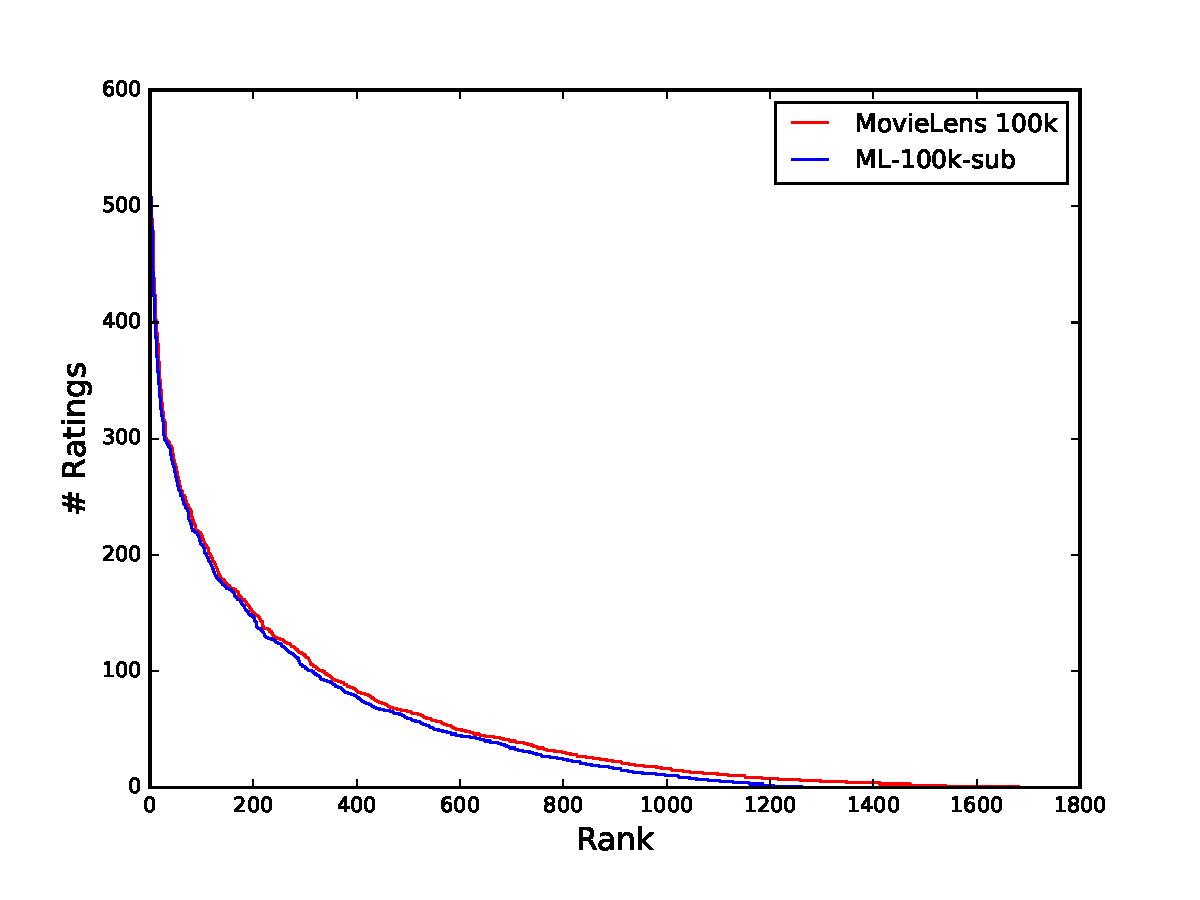
\includegraphics[width=0.7\linewidth]{./section-chapter2/figures/ml-100k_tail.pdf}
	\caption{Rank-size distribution of the MovieLens 100k and ML-100k-sub datasets}
	\label{f:ml-100k-tail}
\end{figure}

\begin{figure}[p]
	\centering
	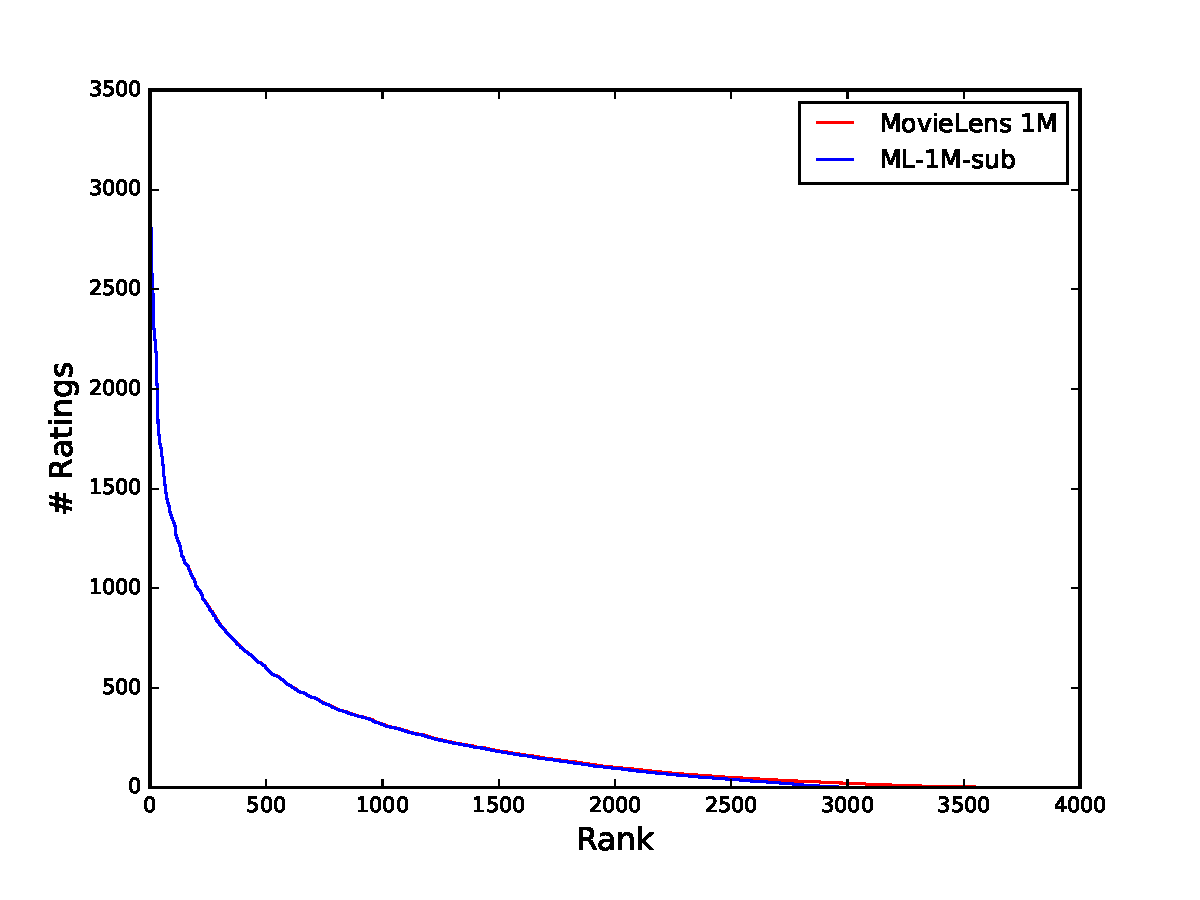
\includegraphics[width=0.7\linewidth]{./section-chapter2/figures/ml-1m_tail.pdf}
	\caption{Rank-size distribution of the MovieLens 1M and ML-1M-sub datasets}
	\label{f:ml-1m-tail}
\end{figure}

\section{Baseline}
\label{st:baseline}

Both the MPCFs-SI (Section \ref{sst:mpcfs-si}) and MFNN (Section \ref{sst:mfnn}) models were compared against three baseline methods.
The baseline recommender consists of the nonlinear matrix factorization model MPCFs discussed in Section \ref{st:mpcf}, a linear recommender called SLIM \cite{Ning2011}, and another state-of-the-art recommender also based on a latent factor model obtained with matrix factorization, called BPRMF \cite{Rendle2009}.

\section{Methodology}
\label{st:methodology}
The standard way of splitting datasets for evaluating recommendation systems is that a percentage of each user's ratings remain in the training set while the rest goes into the test set.
However, datasets have been subdivided, such that 70\% of each movie's ratings were used for training, and the rest for testing.
The rational explanation of this method of splitting the sample is to make the movie data especially sparse.
We were also making sure that each user has at least one rating in the test set in order to measure the performance.

For each recommender, a parameter grid was defined and 12 or more parameter sets were randomly drawn from that grid.
The parameter set which resulted in the best area under the ROC curve (AUC) for each model was then selected.
The best parameter sets are listed in Appendix \ref{a:best-params}.
The performance of the methods was then evaluated using five different randomly drawn splits in a manner described in the previous paragraph.

Measures were reported after 20 iterations for MPCFs, MPCFs-SI, and BPRMF.
The number of iterations for the SLIM model was a hyperparameter.
We have found that five epochs give us the best results.
Our model MFNN is computationally quite expensive and takes a lot of time.
We also ran 20 iterations of the MFNN model on the ML-100k-sub, however, we had to limit the number of iterations of that model for the ML-1M-sub dataset to 10 epochs.

\section{Performance Measures}
\label{st:performance-measures}
We use the area under the ROC curve (AUC) as our main measure to evaluate each approach.
Moreover, we have adopted several commonly used measures to evaluate the performance of the recommender.
The following measures were calculated: area under the ROC curve (AUC), Precision@20 (P@20), Recall@20 (R@20), Mean Reciprocal Rank (MRR) and Spearman Rank Correlation (SRC).
Furthermore, we have carried out an additional measure related to AUC: Instead of recommending items to users and calculate the ranking measure, we were recommending users to items and calculating the rank measure for each item.
This is called IAUC.


\section{Performance Comparison}
\label{st:performance-comparison}


Measures were defined in Section \ref{st:performance-measures} and used to determine the performance of the models introduced in Section \ref{st:using-extra-data} as well as the baseline recommender.
MPCFs-SI performs better on all calculated performance measures on ML-100k-sub compared to the best baseline recommender, which is MPCFs.
On ML-1M-sub, MPCFs-SI is superior to MPCFs in terms of AUC, IAUC and Spearman Rank Correlation.
Results show that MFNN is inferior to \text{MPCFs} on all measures except Precision@20 and Recall@20 on the ML-100k-sub dataset.
MFNN is performing at a similar level as MPCFs-SI regarding AUC and has the best Spearman Rank Correlation of all recommender on the bigger ML-1M-sub.
The full results are summarized in Table \ref{tab:performance}.

Table \ref{tab:item-factor-sim} presents that similar movies have a high cosine similarity (defined in Eq. \ref{eq:cosine-sim}) in the document vector space.
In fact, the sequels to the listed movies were the most or second most similar movie in that space.
Moreover, looking at the item latent vector space, results show that using MPCFs-SI improves the cosine similarity of all similar items compared to using MPCFs.
The most dissimilar movies in the document vector space of the first listed movies are also analyzed.
MPCFs-SI also separates dissimilars apart and thus decreases the cosine similarity of those movies.
MFNN seems to make all listed movies more similar, irregardless of them being similar in the document vector space or not.
The best performing models on the ML-1M-sub dataset were used to calculate the cosine similarities in Table \ref{tab:item-factor-sim}.

One of our goals was also addressing the cold-start problem.
Our hypothesis here is that incorporating side information would lead to better recommendations for users who have very few ratings.
Figures \ref{f:ml-100k-comp-auc} (ML-100k-sub dataset) and \ref{f:ml-1m-comp-auc} (ML-1M-sub dataset) show the average AUC for a group of users as users with more training ratings were included into that group.

It is surprising that the average AUC goes down the more users with many training ratings are being included in Figure \ref{f:ml-100k-comp-auc}.
However, this must be caused by an inherent characteristic of the ML-100k-sub dataset as that trend is seen for all recommender.
We do not observe that using MPCFs-SI or MFNN improve the AUC for users who have very few ratings on the ML-100k-sub dataset.

On the bigger ML-1M-sub dataset, Figure \ref{f:ml-1m-comp-auc} and Figure \ref{f:ml-1m-comp-auc-zoom} (the zoomed version thereof) indicate that the MFNN model is superior to the other recommender in terms of AUC for users with less than 200 training ratings in particular.
However, MPCFs-SI seems to have an advantage for users with less than 10 training ratings.

For the sake of completeness, the progressions of the average of the other defined measures are presented in Figures \ref{f:ml-100k-comp-iauc} and \ref{f:ml-100k-comp-group} for the ML-100k-sub dataset, and in Figures \ref{f:ml-1m-comp-iauc} and \ref{f:ml-1m-comp-group} for the ML-1M-sub dataset.
\begin{table}[p]
	\begin{center}
		\begin{tabularx}{\linewidth}{cXcccccc}
			\hline \hline
			& \textbf{Method} & \textbf{AUC} & \textbf{IAUC} & \textbf{P@20} & \textbf{R@20} & \textbf{MRR} & \textbf{SRC}\\
			\hline
			\parbox[t]{2mm}{\multirow{7}{*}{\rotatebox[origin=c]{90}{ML-100k-sub}}} & Perfect & 100.0 & 100.0 & 100.0 & 100.0 & 1.0 & 1.0\\
			& MPCFs-SI & \textbf{93.76} & \textbf{90.83} & 28.16 & \textbf{44.27} & \textbf{0.6866} & \textbf{0.2005}\\
			& MFNN & 93.48 & 89.74 & \textbf{28.44} & 43.96 & 0.6741 & 0.1925 \\
			& \multicolumn{7}{c}{\hdashrule[0.5ex][c]{14cm}{0.5pt}{1mm}} \\
			& MPCFs & 93.65 & 90.78 & 27.79 & 43.55 & 0.6770 & 0.1974 \\
			& BPRMF & 92.20 & 68.03 & 18.00 & 27.38 & 0.3703 & 0.1567 \\
			& SLIM & 91.45 & 85.20 & 23.49 & 37.75 & 0.5993 & 0.1880 \\
			\hline
			\parbox[t]{2mm}{\multirow{7}{*}{\rotatebox[origin=c]{90}{ML-1M-sub}}} & Perfect & 100.0 & 100.0 & 100.0 & 100.0 & 1.0 & 1.0\\
			& MPCFs-SI & 92.88 & \textbf{92.15} & 32.11 & 32.77 & 0.6941 & 0.2260 \\
			& MFNN & \textbf{92.89} & 91.73 & 30.36 & 29.54 & 0.6481 & \textbf{0.2351} \\
			& \multicolumn{7}{c}{\hdashrule[0.5ex][c]{14cm}{0.5pt}{1mm}} \\
			& MPCFs & 92.81 & 92.08 & \textbf{32.71} & \textbf{33.44} & \textbf{0.7035} & 0.2223 \\
			& BPRMF & 91.82 & 67.54 & 21.23 & 20.13 & 0.4430 & 0.2013 \\
			& SLIM & 91.23 & 88.00 & 28.59 & 28.76 & 0.6465 &  0.2322 \\
			\hline \hline
		\end{tabularx}
	\end{center}
	\caption{Performance measures. The best result for each measure and dataset is highlighted in bold.}
	\label{tab:performance}
\end{table}


\begin{table}[p]
	\begin{center}
		\begin{tabularx}{\linewidth}{XXcccc}
			\hline \hline
			\textbf{Movie 1} & \textbf{Movie 2} & \textbf{Doc2Vec} & \textbf{MPCFs} & \textbf{MPCFs-SI} & \textbf{MFNN} \\
			\hline
			Free Willy & Free Willy 2 & 0.8694 & 0.6915 & 0.7329 & 0.8305\\
			Jurassic Park & Jurassic Park 2 & 0.6796 & 0.5418 & 0.6214 & 0.7440\\
			Scream & Scream 2 & 0.7514 & 0.7016 & 0.7362 & 0.8325\\
			Species & Species II & 0.6831 & 0.6641 & 0.7015 & 0.8203\\
			Star Wars V & Star Wars VI & 0.9231 & 0.6846 & 0.7650 & 0.8717\\
			Toy Story & Toy Story 2 & 0.7529 & 0.6546 & 0.6838 & 0.7929\\
			\hline
			Free Willy & Mrs. Brown & -0.0141 & -0.0366 & -0.0927 & 0.0977\\
			Jurassic Park & Battling Butler & -0.1127 & -0.1218 & -0.1805 & -0.0083\\
			Scream & Kelly's Heroes & -0.0465 & -0.1385 & -0.1971 & -0.0868\\
			Species & Patton & -0.0763 & -0.0283 & -0.0485 & 0.0942\\
			Star Wars V & Angela's Ashes & -0.0130 & -0.1433 & -0.1732 & -0.1183\\
			Toy Story & Raise the Red Lantern & -0.0257 & -0.0256 & -0.0490 & 0.0593\\
			\hline \hline
		\end{tabularx}
	\end{center}
	\caption{Item cosine similarities, measured in the document vector space and the item latent vector space of the according model.}
	\label{tab:item-factor-sim}
\end{table}


\begin{figure}[p]
	\centering
	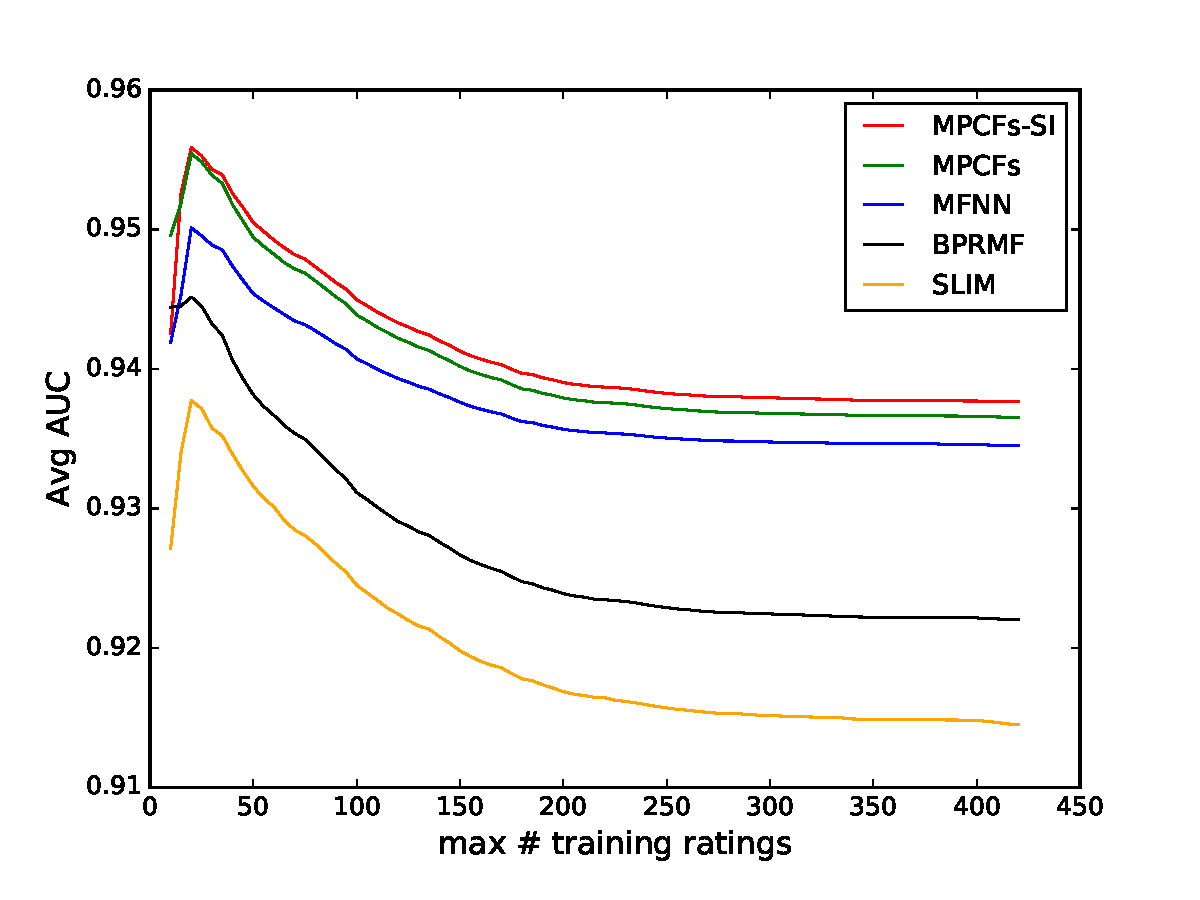
\includegraphics[width=0.7\linewidth]{./section-chapter2/figures/ml-100k_comparison_auc.pdf}
	\caption{Average AUC for a group of users as users with more training ratings were included into that group.
		The performance is measured on the ML-100k-sub dataset.}
	\label{f:ml-100k-comp-auc}
\end{figure}

\begin{figure}[p]
	\centering
	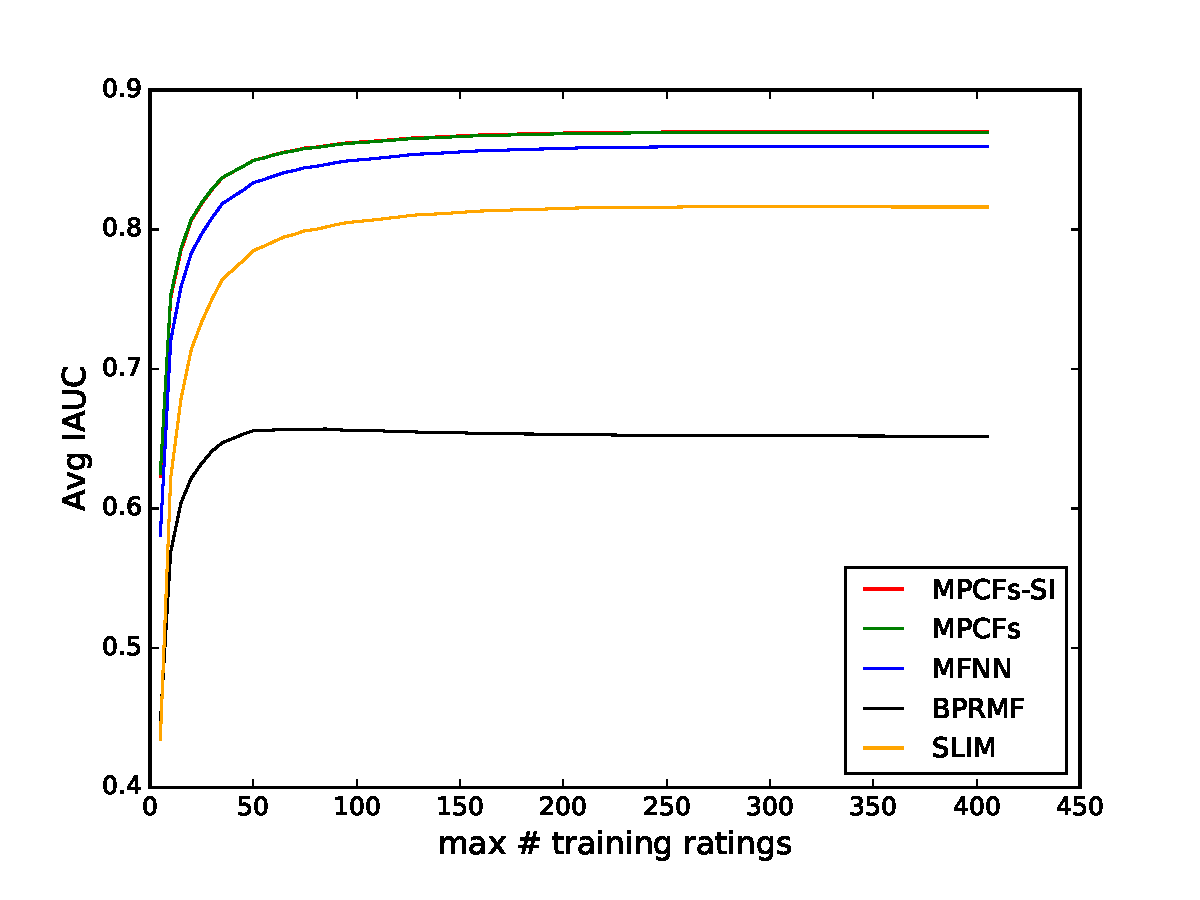
\includegraphics[width=0.7\linewidth]{./section-chapter2/figures/ml-100k_comparison_iauc.pdf}
	\caption{Average IAUC for a group of users as users with more training ratings were included into that group.
		The performance is measured on the ML-100k-sub dataset.}
	\label{f:ml-100k-comp-iauc}
\end{figure}

\begin{figure}
	\centering
	\begin{subfigure}[b]{0.46\linewidth}
		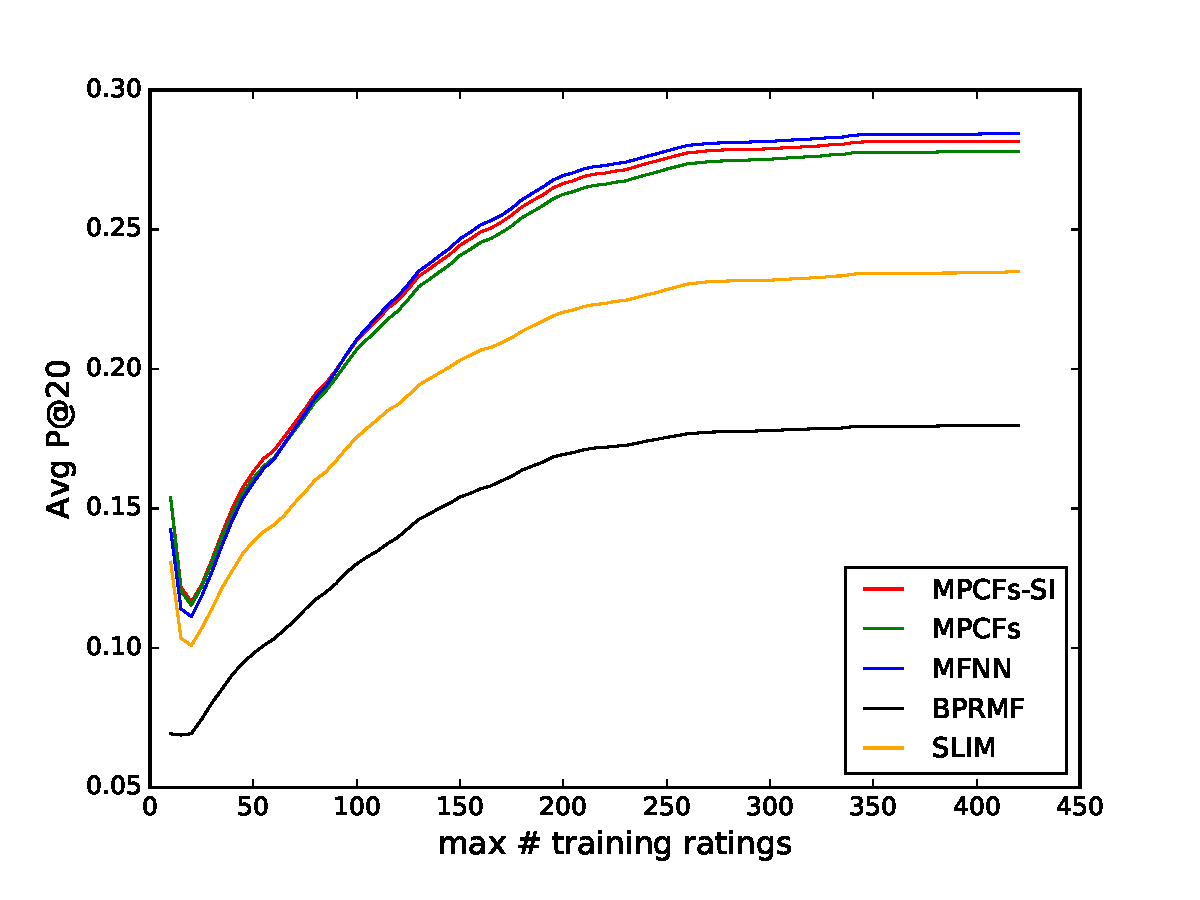
\includegraphics[width=\linewidth]{./section-chapter2/figures/ml-100k_comparison_p20.pdf}
	\end{subfigure}
	\begin{subfigure}[b]{0.46\linewidth}
		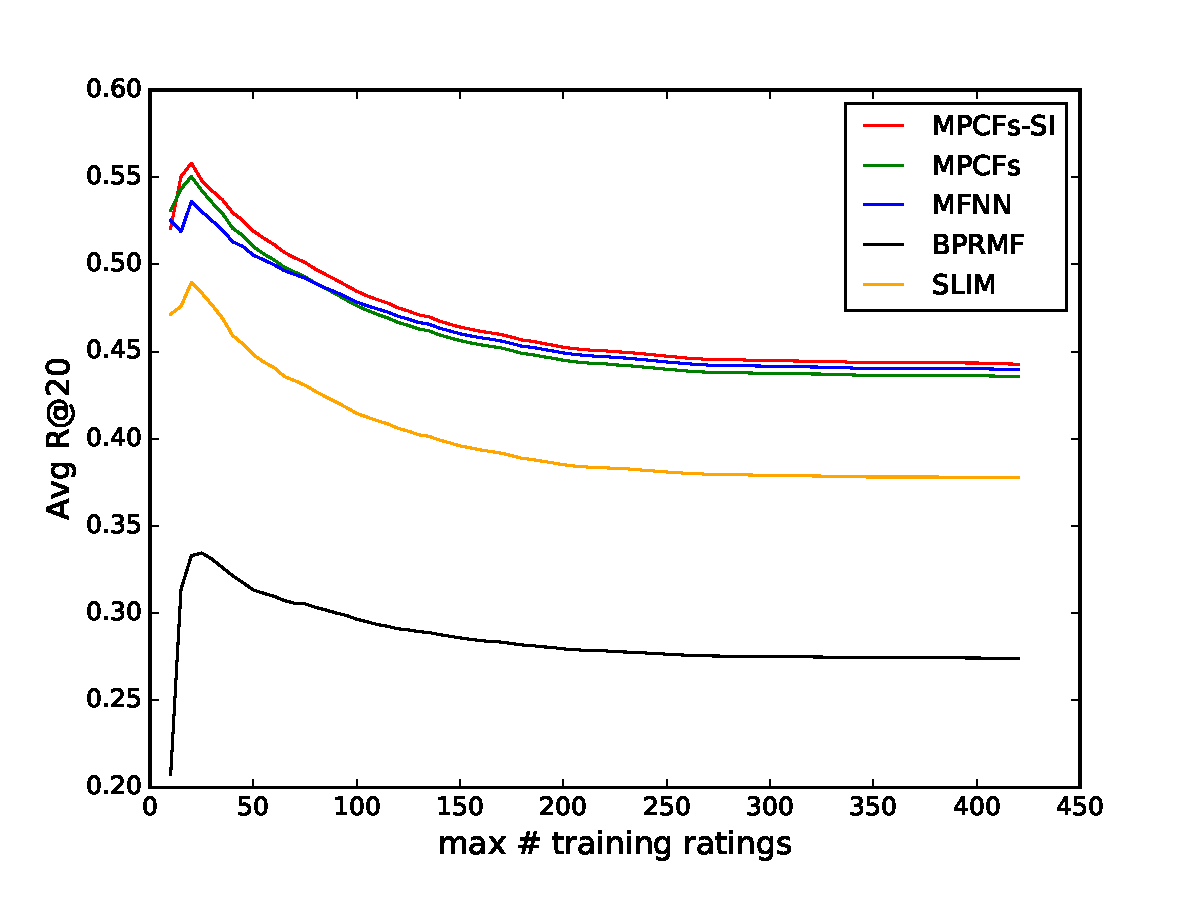
\includegraphics[width=\linewidth]{./section-chapter2/figures/ml-100k_comparison_r20.pdf}
	\end{subfigure}
	\begin{subfigure}[b]{0.46\linewidth}
		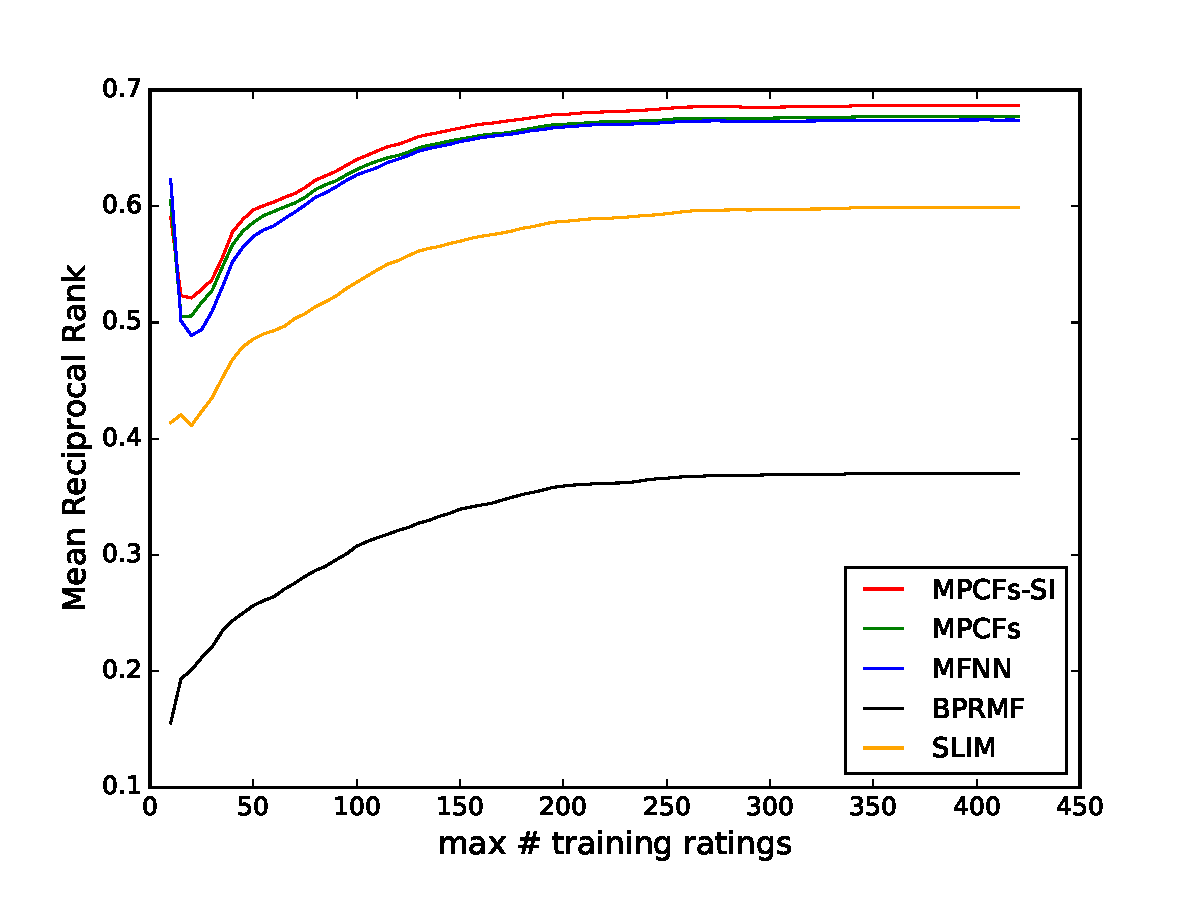
\includegraphics[width=\linewidth]{./section-chapter2/figures/ml-100k_comparison_mrr.pdf}
	\end{subfigure}
	\begin{subfigure}[b]{0.46\linewidth}
		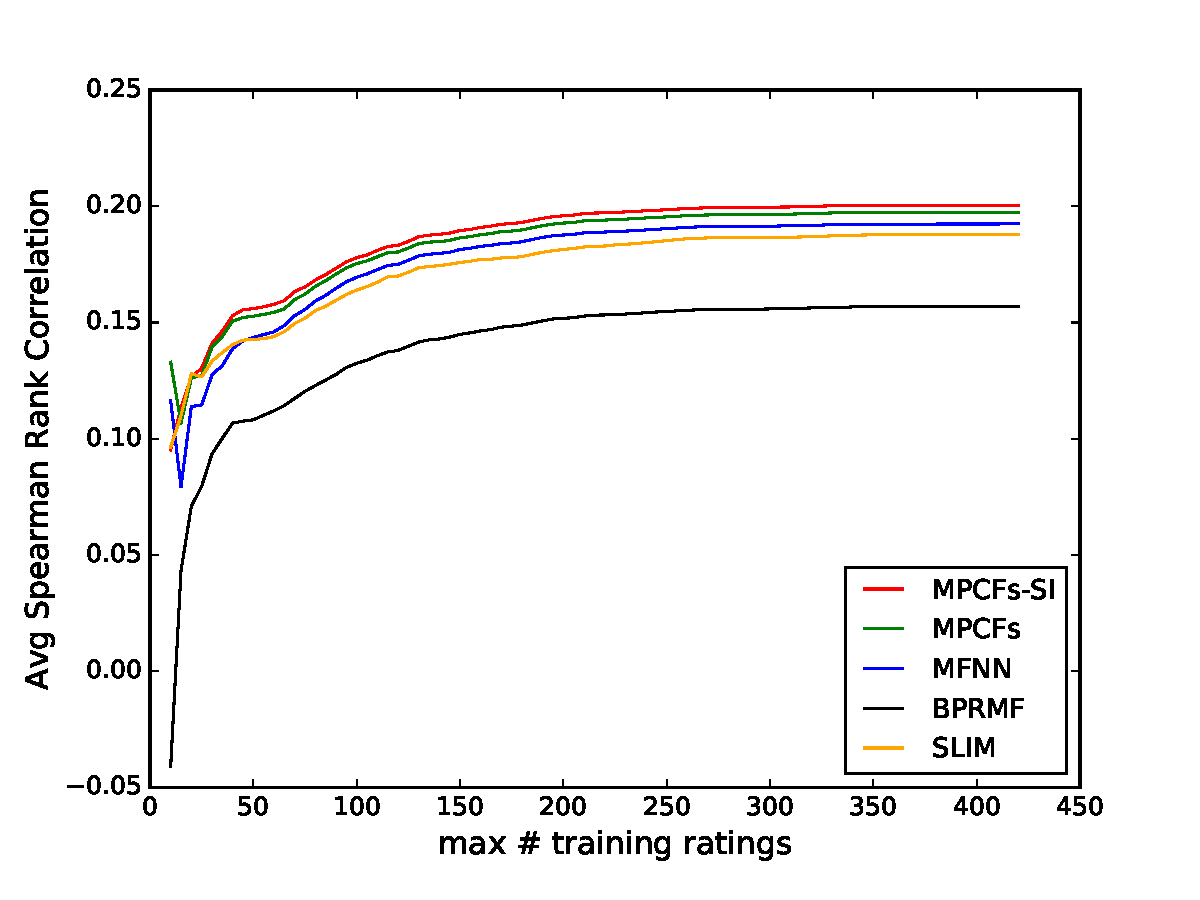
\includegraphics[width=\linewidth]{./section-chapter2/figures/ml-100k_comparison_src.pdf}
	\end{subfigure}
	
	\caption{Measured on the ML-100k-sub dataset.}
	\label{f:ml-100k-comp-group}
\end{figure}


\begin{figure}[p]
	\centering
	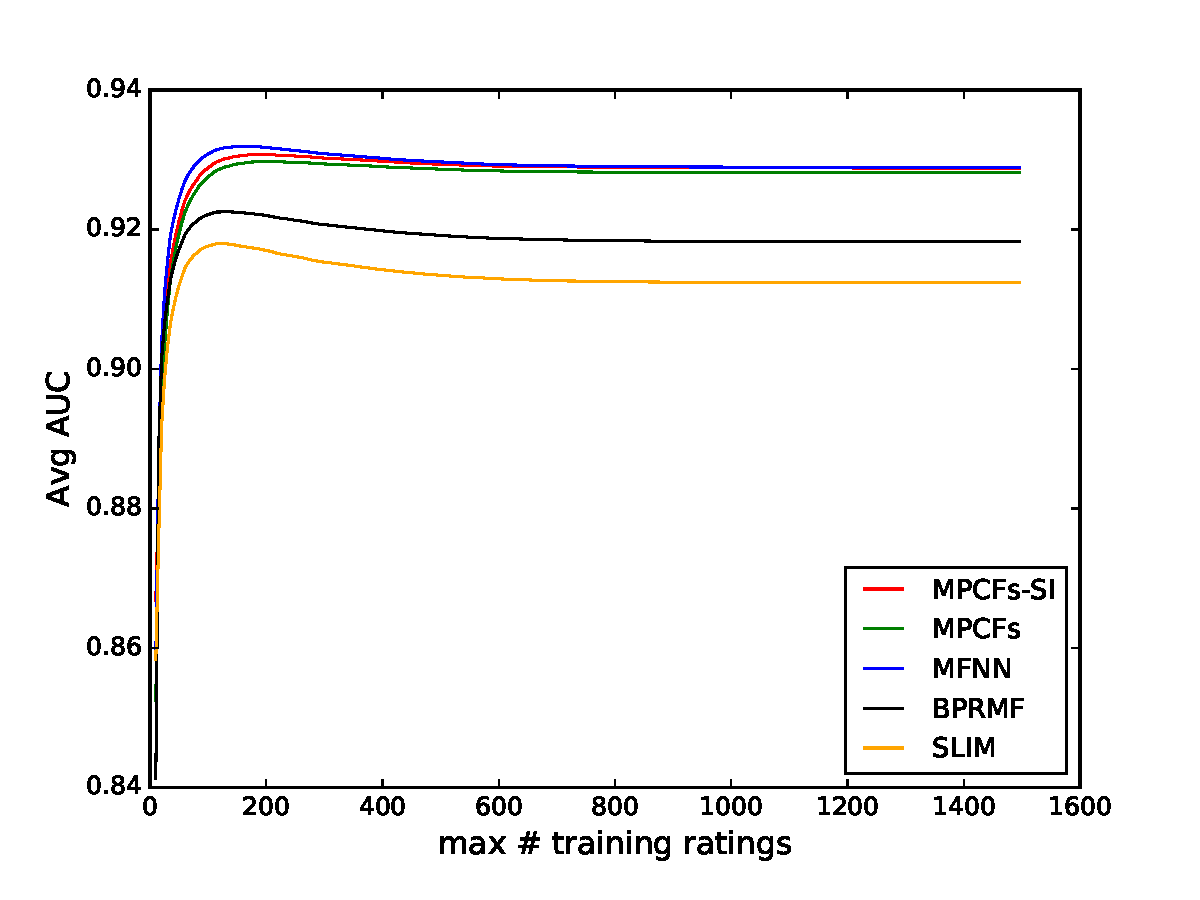
\includegraphics[width=0.7\linewidth]{./section-chapter2/figures/ml-1m_comparison_auc.pdf}
	\caption{
		Average AUC for a group of users as users with more training ratings were included into that group.
		The performance is measured on the ML-1M-sub dataset.}
	\label{f:ml-1m-comp-auc}
\end{figure}

\begin{figure}[p]
	\centering
	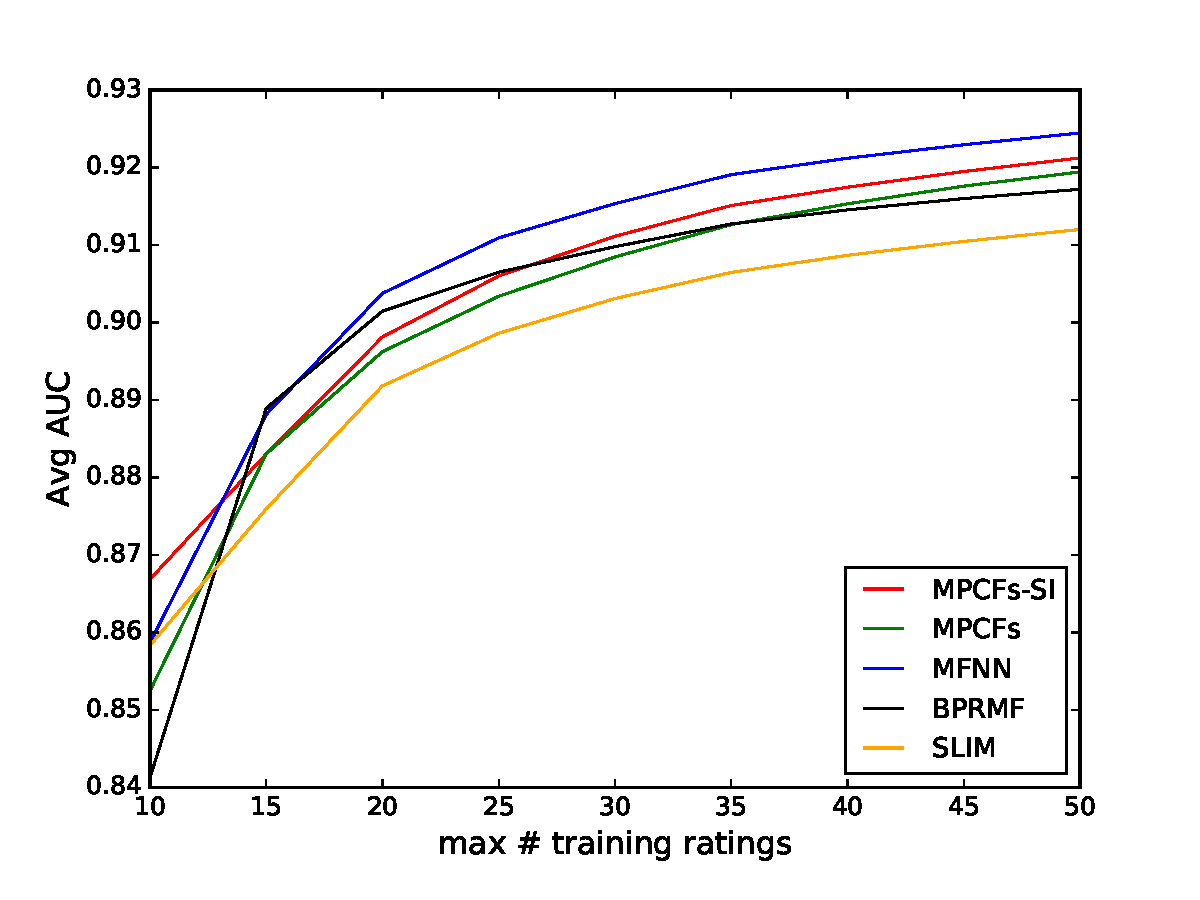
\includegraphics[width=0.7\linewidth]{./section-chapter2/figures/ml-1m_comparison_auc_zoom.pdf}
	\caption{Average AUC for a group of users as users with more training ratings were included into that group.
		The performance is measured on the ML-1M-sub dataset.
		Zoomed version of Figure \ref{f:ml-1m-comp-auc}.}
	\label{f:ml-1m-comp-auc-zoom}
\end{figure}

\begin{figure}[p]
	\centering
	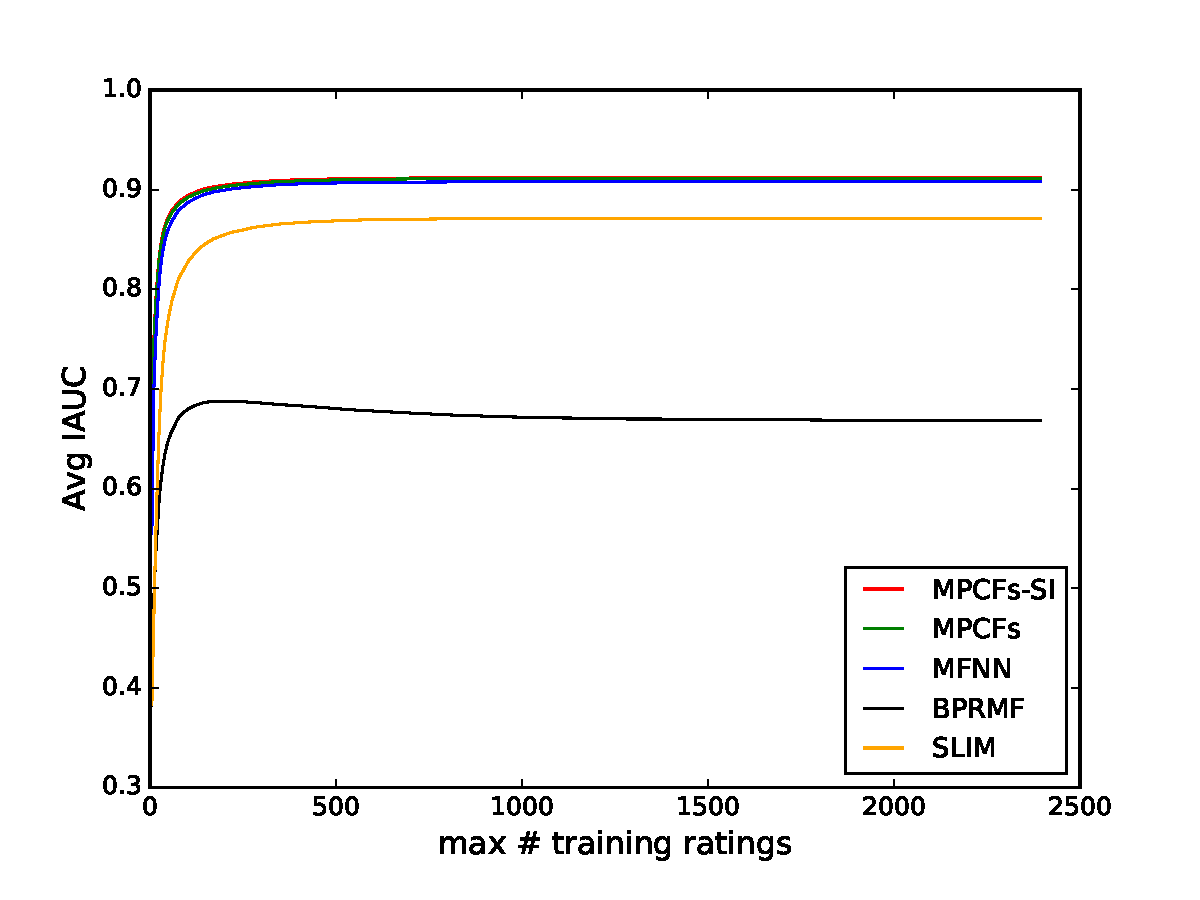
\includegraphics[width=0.7\linewidth]{./section-chapter2/figures/ml-1m_comparison_iauc.pdf}
	\caption{
		Average IAUC for a group of users as users with more training ratings were included into that group.
		The performance is measured on the ML-1M-sub dataset.}
	\label{f:ml-1m-comp-iauc}
\end{figure}

\begin{figure}
	\centering
	\begin{subfigure}[b]{0.46\linewidth}
		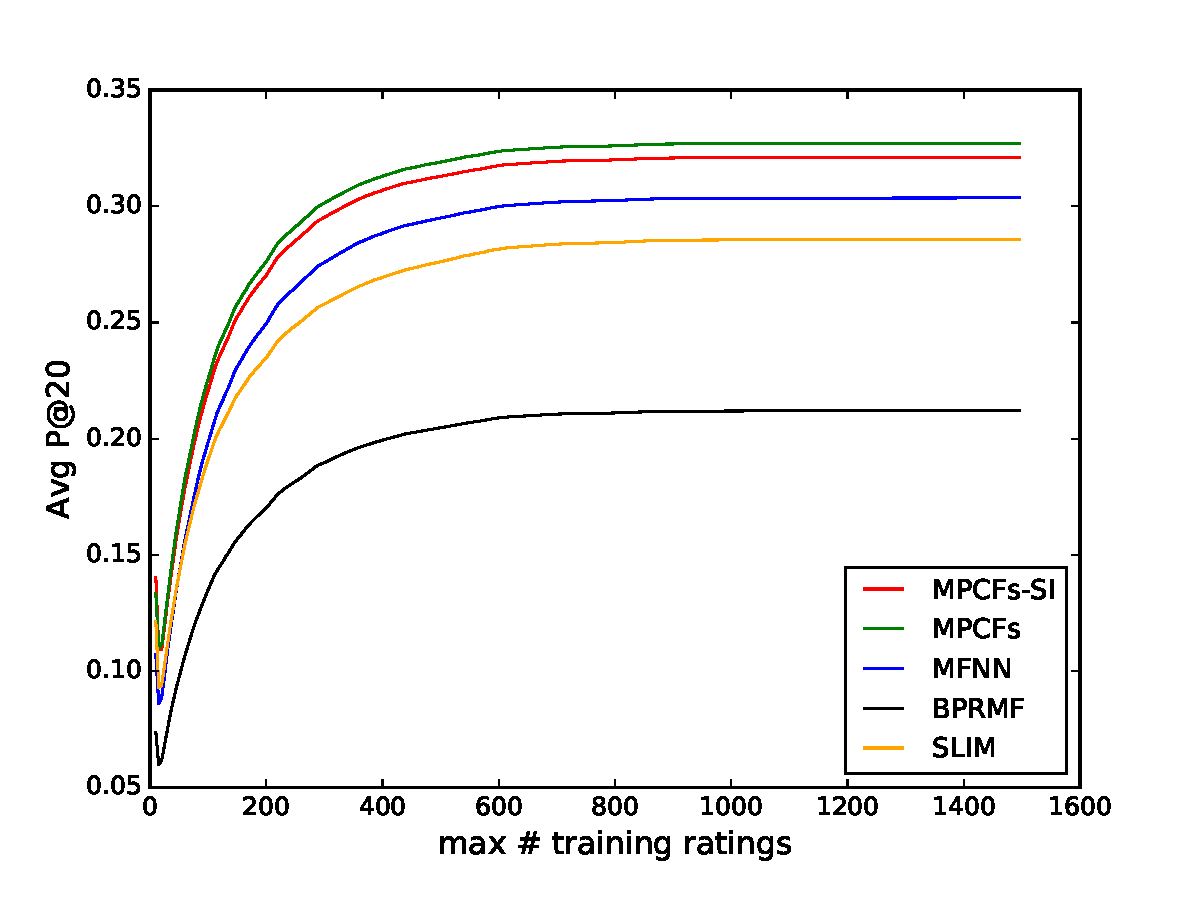
\includegraphics[width=\linewidth]{./section-chapter2/figures/ml-1m_comparison_p20.pdf}
	\end{subfigure}
	\begin{subfigure}[b]{0.46\linewidth}
		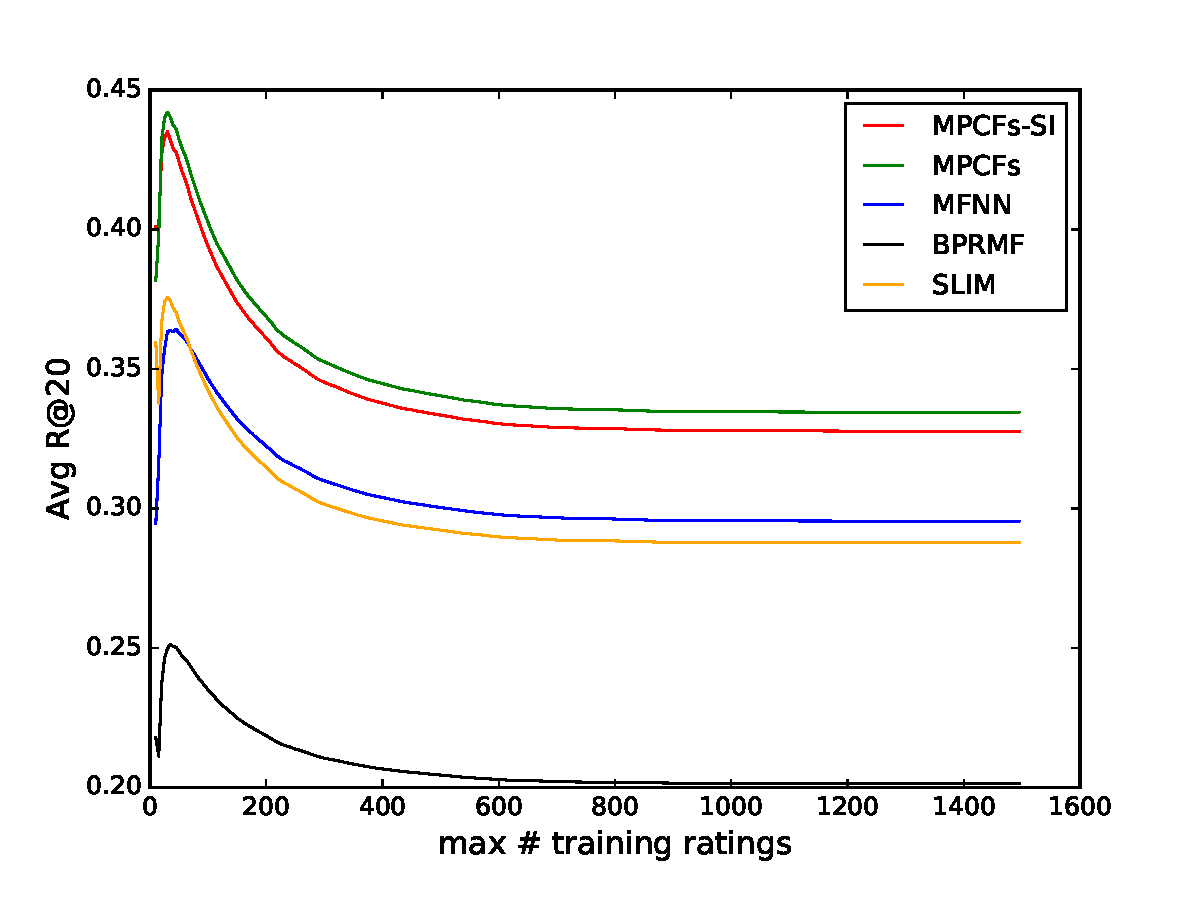
\includegraphics[width=\linewidth]{./section-chapter2/figures/ml-1m_comparison_r20.pdf}
	\end{subfigure}
	\begin{subfigure}[b]{0.46\linewidth}
		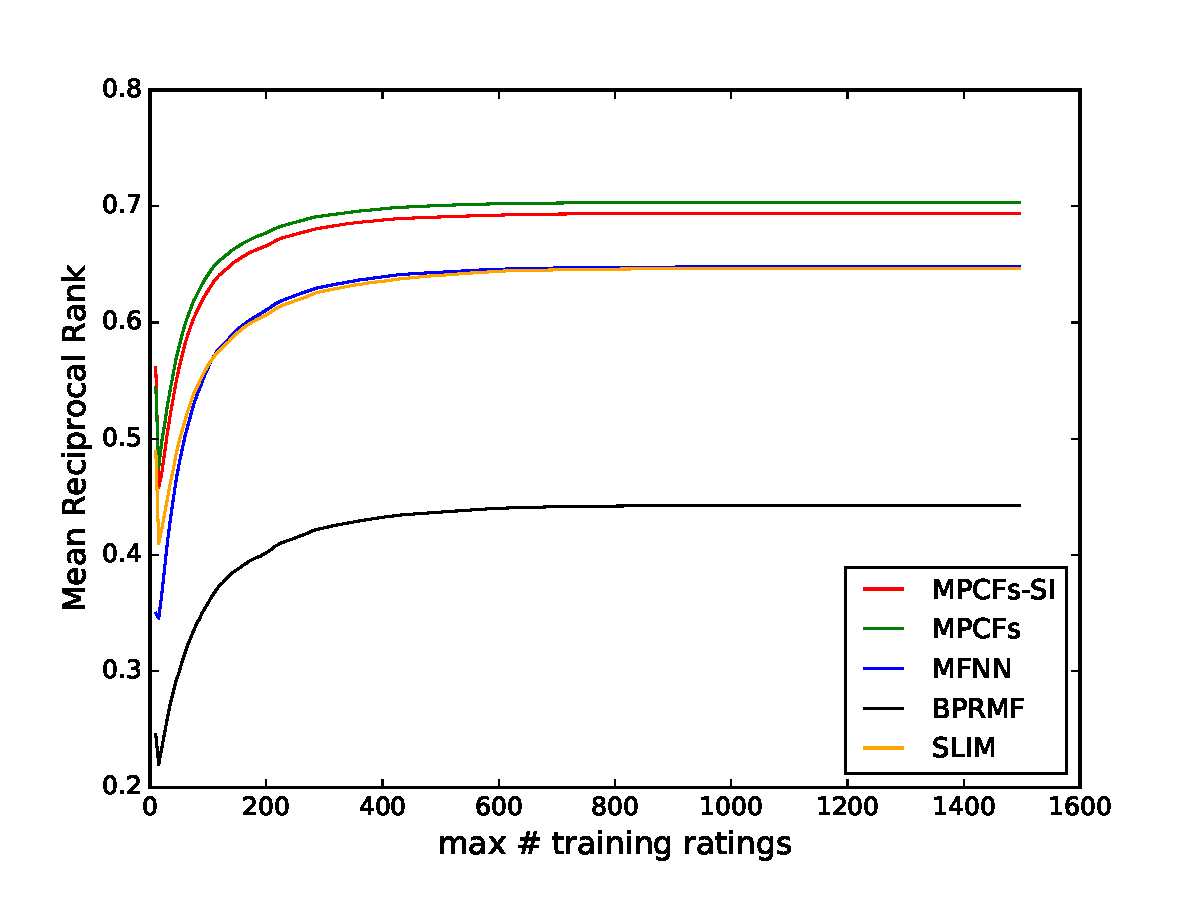
\includegraphics[width=\linewidth]{./section-chapter2/figures/ml-1m_comparison_mrr.pdf}
	\end{subfigure}
	\begin{subfigure}[b]{0.46\linewidth}
		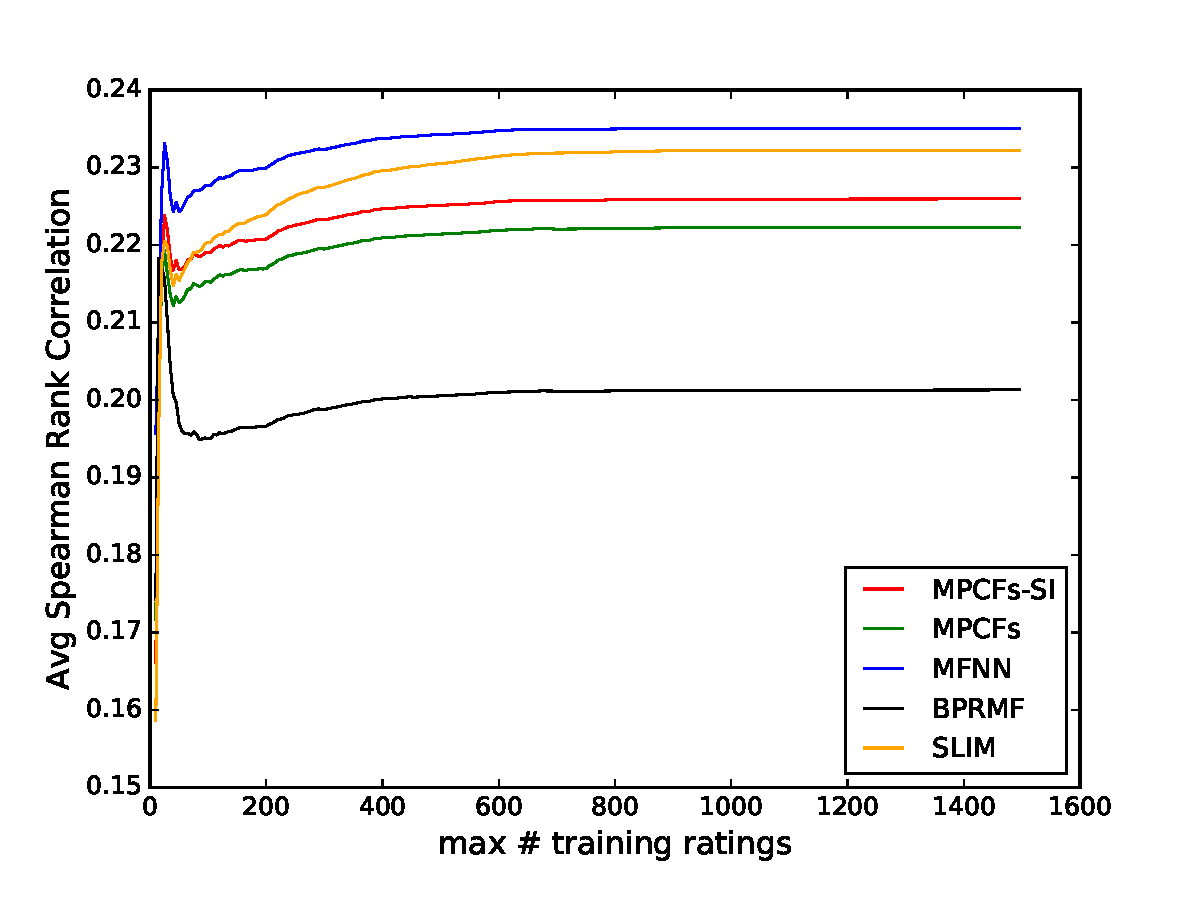
\includegraphics[width=\linewidth]{./section-chapter2/figures/ml-1m_comparison_src.pdf}
	\end{subfigure}
	
	\caption{Measured on the ML-1M-sub dataset.}
	\label{f:ml-1m-comp-group}
\end{figure}
\newpage
\section{System Setup}
\label{st:system-setup} 

A custom software was built in Python.
Our two models, MPCFs-SI and MFNN, as well as the baseline recommender MPCFs \cite{Kabbur2015} and BPRMF \cite{Rendle2009} were implemented by us.
For the baseline recommender SLIM \cite{Ning2011}, we were able to use parts of an open source implementation by Mendeley\footnote{Mendeley mrec - https://github.com/Mendeley/mrec}.
Data handling was done with the Pandas library\footnote{Pandas - http://pandas.pydata.org/} and we have used Numpy\footnote{Numpy - http://www.numpy.org/} for linear algebra operations.
As explained in Section \ref{sst:feature-extraction}, feature vectors for the movies were extracted from their subtitles with the help of Gensim\footnote{Gensim - https://radimrehurek.com/gensim/} and NLTK\footnote{NLTK - http://www.nltk.org/}.
The affine transformation of the MPCFs-SI model, as well as the neural network of the MFNN model, were implemented with Lasagne\footnote{Lasagne - https://github.com/Lasagne/Lasagne} and Theano\footnote{Theano - http://deeplearning.net/software/theano/}.
The source code for this work can be downloaded under https://github.com/marcuniq/bsc-thesis.
